% Relatório da calibração de câmera. Compile a partir desta pasta:
%   latexmk -pdf relatorio.tex && cp relatorio.pdf ../RELATORIO.pdf
\documentclass[10pt,a4paper]{article}

\usepackage[utf8]{inputenc}
\usepackage[T1]{fontenc}
\usepackage[brazilian]{babel}
\usepackage[margin=1.8cm]{geometry}
\usepackage{amsmath}
\usepackage{graphicx}
\usepackage{booktabs}
\usepackage[hidelinks]{hyperref}
\usepackage{titlesec}
\usepackage{enumitem}
\titlespacing*{\section}{0pt}{6pt}{2pt}
\titlespacing*{\subsection}{0pt}{4pt}{2pt}
\setlength{\parskip}{2pt}
\setlist{nosep}
\graphicspath{{../resultados/}}

\title{\vspace{-1.6cm}Calibração de câmera e projeção de pontos 3D}
\author{Gustavo Jakobi (GRR20221253) \quad Bruno Crestani (GRR20221240)\\
  \small Visão Computacional -- Universidade Federal do Paraná -- 2026\\
  \small Repositório: \url{https://github.com/BrunoCrestani/syncingCamera}}
\date{\vspace{-1.2cm}}

\begin{document}
\maketitle

\section*{Método}

Calibramos a câmera principal (1$\times$) de um iPhone 16 Pro (lente de
6,765~mm, f/1.78, equivalente a 24~mm) pelo método de Zhang~\cite{zhang}, com o
OpenCV~\cite{opencv}. O tabuleiro do VRI tem $8\times8$ quadrados, ou seja,
$7\times7$ cantos internos. Não medimos o lado do quadrado; por isso, as
coordenadas 3D estão em \textbf{unidades de quadrado}. Isso não altera $K$ nem
a distorção.

As 19 fotos ($4536\times8064$, retrato) foram reduzidas para $1134\times2016$,
com o mesmo fator e sem recorte. Quatro fotos foram reservadas para validação
antes da calibração. O detector encontrou o tabuleiro em 14 fotos: 10 de
calibração e 4 de validação. As outras 5 têm o tabuleiro cortado pela borda da
foto ou reflexos fortes.

O modelo de projeção é $s\,[u, v, 1]^T = K\,[R\,|\,\mathbf{t}]\,[X, Y, Z, 1]^T$,
com distorção radial e tangencial aplicada às coordenadas normalizadas. O mundo
fica no tabuleiro: origem no primeiro canto, $Z=0$ no plano do tabuleiro.

\begin{enumerate}
  \item \texttt{findChessboardCorners} e \texttt{cornerSubPix} localizam os
    cantos. Uma homografia confere cada detecção e rejeita cantos presos em
    reflexos.
  \item \texttt{calibrateCamera} estima $K$ e a distorção. Usamos o modelo
    \texttt{radial1} ($k_1, p_1, p_2$; $k_2 = k_3 = 0$).
  \item \texttt{getOptimalNewCameraMatrix} ($\alpha = 1$) e \texttt{undistort}
    removem a distorção.
  \item Nas fotos de validação, \texttt{solvePnP} estima $R$ e $\mathbf{t}$ com
    metade dos cantos (padrão xadrez). \texttt{projectPoints} projeta a outra
    metade, que comparamos com os cantos detectados. Também projetamos um cubo
    com $Z \neq 0$.
\end{enumerate}

\section*{Resultados}

O RMS de reprojeção da calibração foi \textbf{0,60~px}, com
\[
K = \begin{bmatrix} 1451{,}95 & 0 & 571{,}29\\ 0 & 1453{,}02 & 976{,}75\\
0 & 0 & 1 \end{bmatrix},\qquad
(k_1, k_2, p_1, p_2, k_3) = (0{,}136;\ 0;\ -0{,}0098;\ 0{,}0006;\ 0).
\]
$f_x \approx f_y$ indica pixels quadrados, e o centro óptico fica perto do
centro da imagem $(567, 1008)$. Pela focal do EXIF, esperávamos
$f_x \approx 1400$~px; a diferença de 4\,\% é compatível com o valor nominal de
24~mm. O modelo completo reduz o RMS só para 0,56~px, mas dá $k_3 = -3{,}33$:
um sinal de sobreajuste, porque o tabuleiro nunca chega às bordas da imagem.

O iPhone já corrige a maior parte da distorção por software, então a correção é
pequena. Para medi-la, ajustamos uma reta a cada linha e coluna de cantos e
calculamos a distância RMS dos cantos à reta (\emph{retitude}). A perspectiva
preserva retas; a curvatura restante vem da lente e do ruído do detector.

\begin{table}[htb]
  \centering\small
  \begin{tabular}{lccccc}
    \toprule
    Foto de validação & Erro médio (px) & RMS (px) & Erro máx. (px) &
    Retitude original (px) & Retitude corrigida (px)\\
    \midrule
    IMG\_8157 & 0,20 & 0,22 & 0,42 & 0,32 & 0,11\\
    IMG\_8165 & 1,01 & 1,25 & 3,65 & 0,64 & 0,62\\
    IMG\_8171 & 0,54 & 0,59 & 0,93 & 0,30 & 0,24\\
    IMG\_8174 & 0,90 & 0,97 & 1,65 & 0,69 & 0,57\\
    \bottomrule
  \end{tabular}
  \caption{Erro entre os 24 cantos de teste projetados e detectados em cada
  foto de validação, e retitude antes e depois de remover a distorção.}
  \label{tab:validacao}
\end{table}

\vspace{-6pt}
\subsection*{Projeção de pontos 3D}

O RMS de validação nos 96 pontos de teste foi \textbf{0,85~px}
(Tabela~\ref{tab:validacao}). A Tabela~\ref{tab:pontos} mostra exemplos; a
tabela completa está em \texttt{resultados/projecoes.csv}.

\begin{table}[htb]
  \centering\small
  \begin{tabular}{lcccc}
    \toprule
    Foto & $X, Y, Z$ (quadrados) & $u, v$ previstos (px) &
    $u, v$ observados (px) & Erro (px)\\
    \midrule
    IMG\_8171 & 1, 0, 0 & 634,3; 630,9 & 634,5; 630,2 & 0,68\\
    IMG\_8171 & 3, 2, 0 & 690,3; 850,5 & 690,1; 850,2 & 0,33\\
    IMG\_8171 & 5, 4, 0 & 741,2; 1046,6 & 740,5; 1046,3 & 0,74\\
    IMG\_8174 & 1, 0, 0 & 500,0; 773,1 & 500,5; 772,8 & 0,59\\
    IMG\_8174 & 3, 2, 0 & 543,7; 914,7 & 544,0; 915,9 & 1,23\\
    IMG\_8174 & 5, 4, 0 & 597,5; 1088,5 & 597,8; 1089,0 & 0,66\\
    \bottomrule
  \end{tabular}
  \caption{Pontos 3D projetados e cantos detectados.}
  \label{tab:pontos}
\end{table}

O cubo tem base de $(1, 1, 0)$ a $(5, 5, 0)$ e altura de 4 quadrados, do lado da
câmera. Por exemplo, em IMG\_8171 o vértice $(1, 1, -4)$ é projetado em
$(603{,}1;\ 767{,}5)$. Os vértices de cima não têm referência medida, então a
conferência do cubo é visual: as arestas verticais convergem para o ponto de
fuga esperado e o topo fica maior que a base nas vistas inclinadas
(Figura~\ref{fig:resultados}).

\begin{figure}[htb]
  \centering
  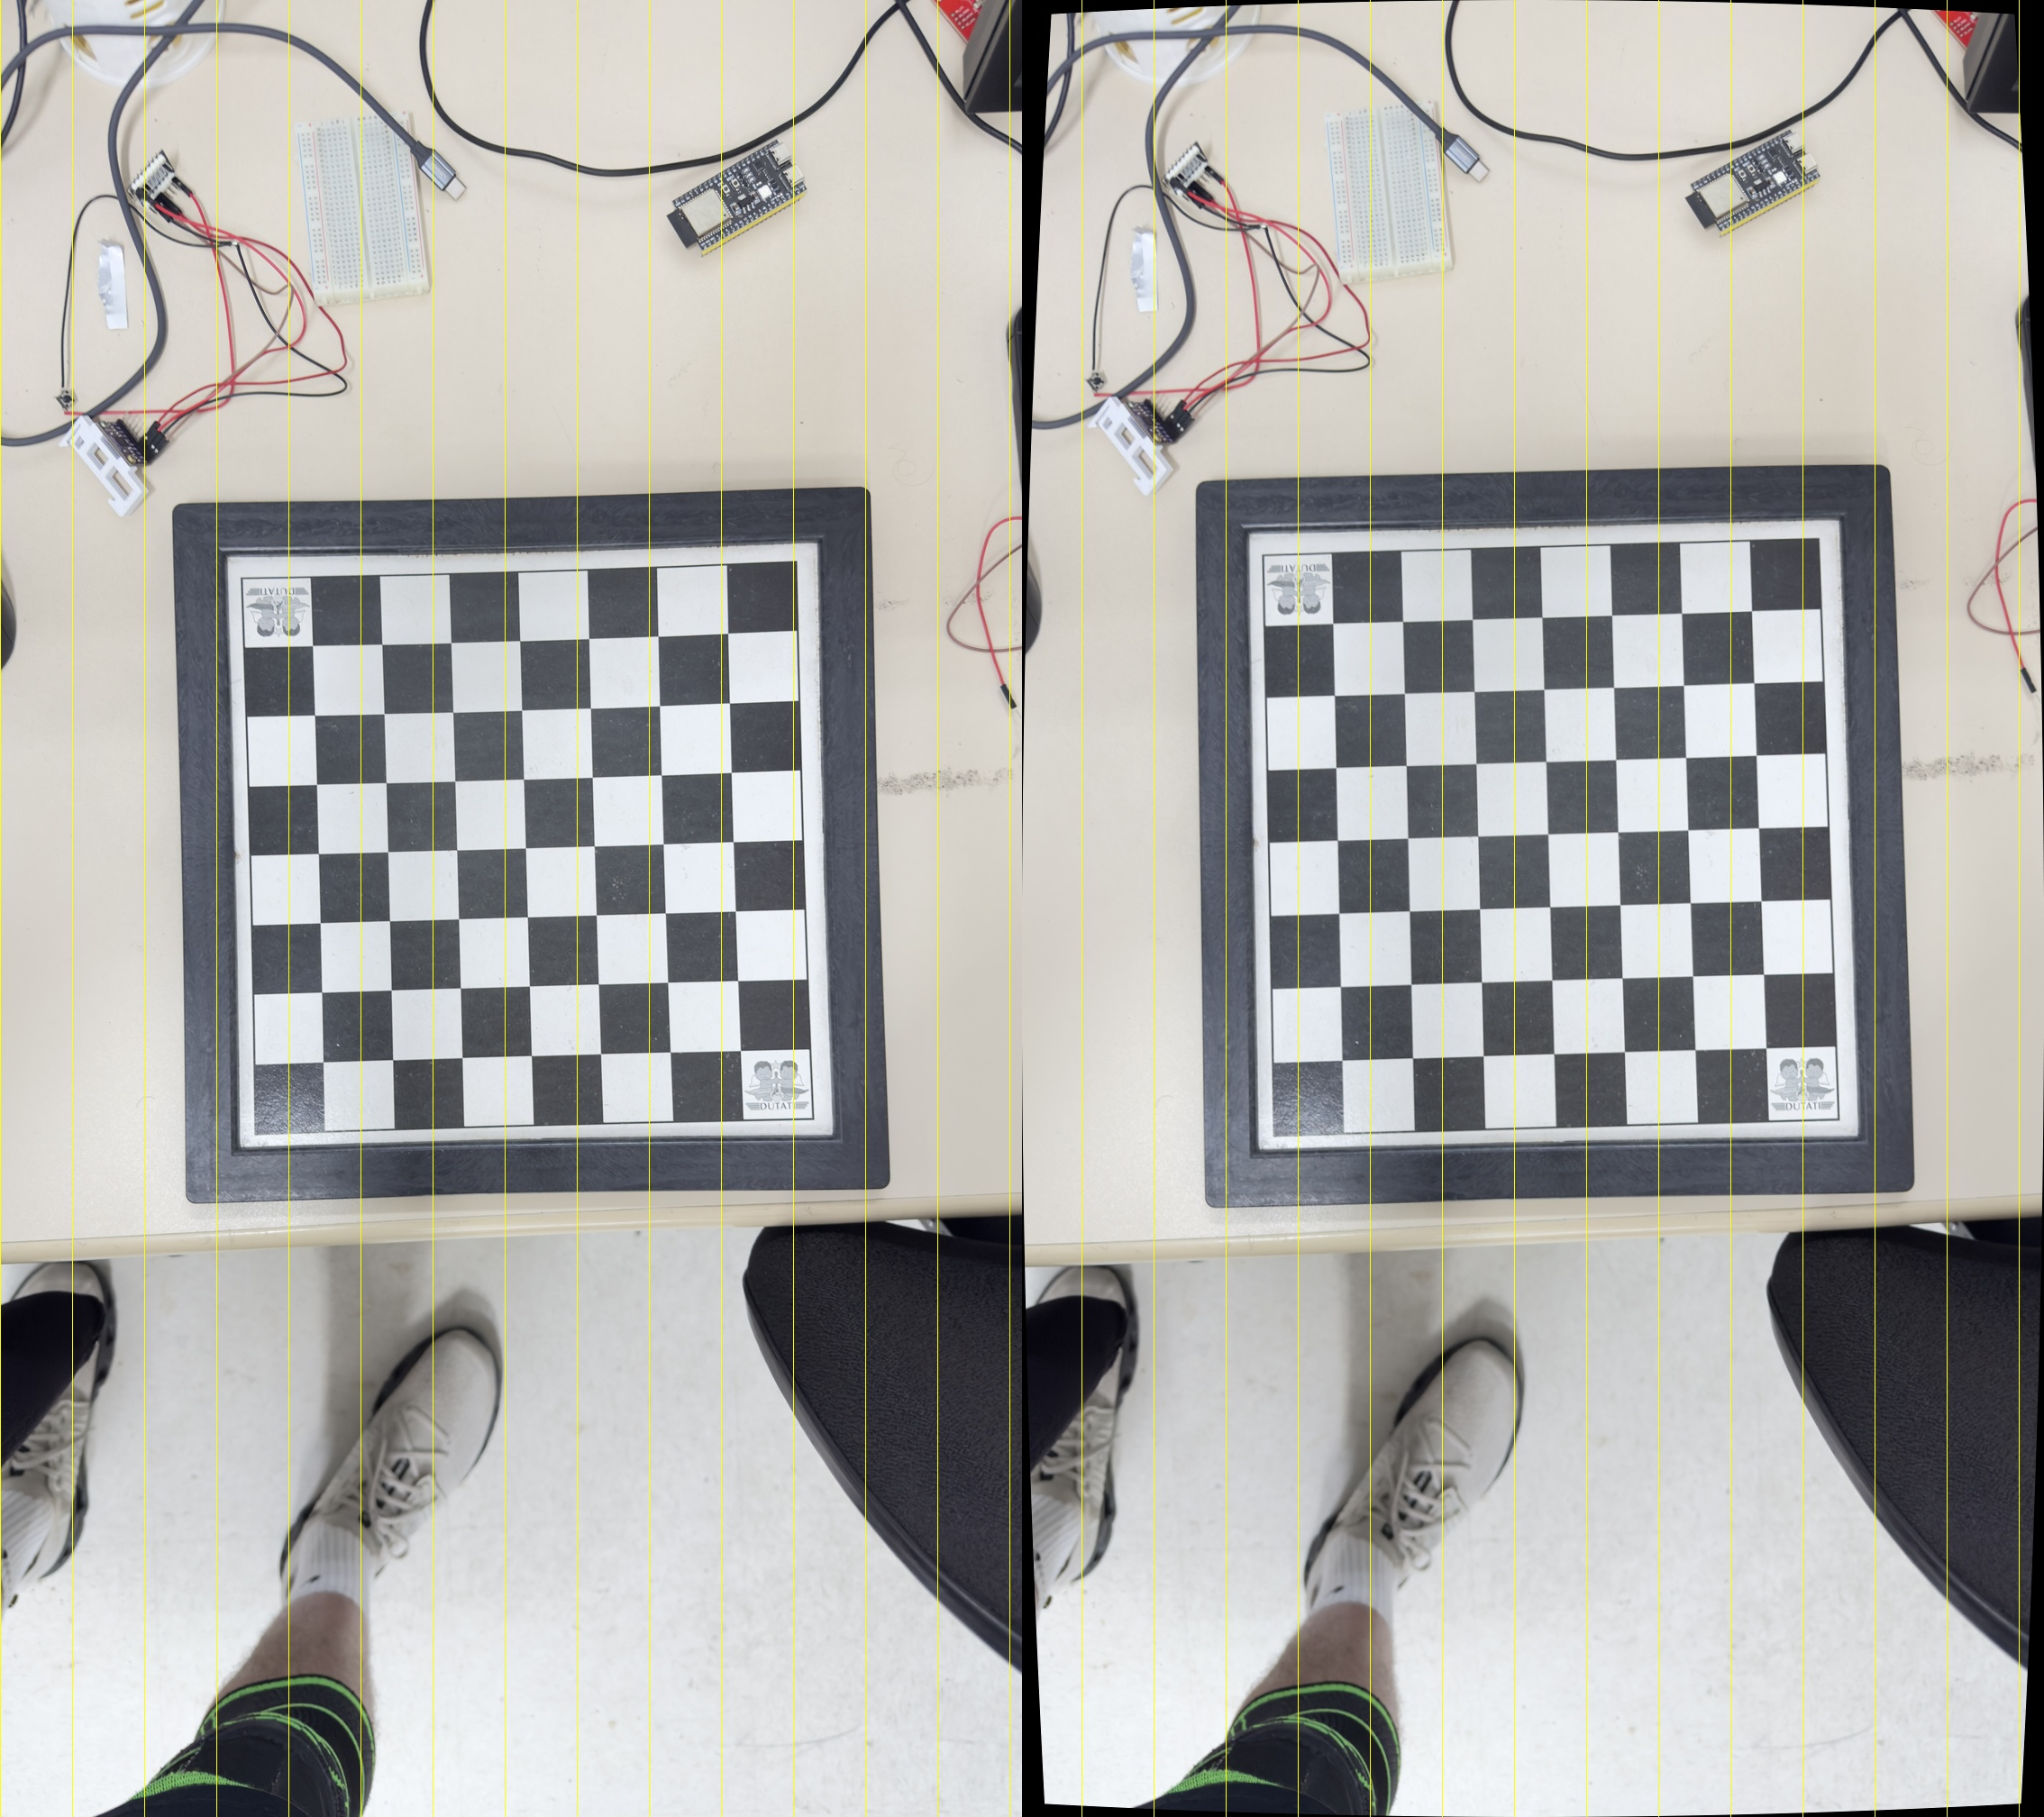
\includegraphics[height=7.2cm]{distorcao_IMG_8157.jpg}\hspace{4mm}%
  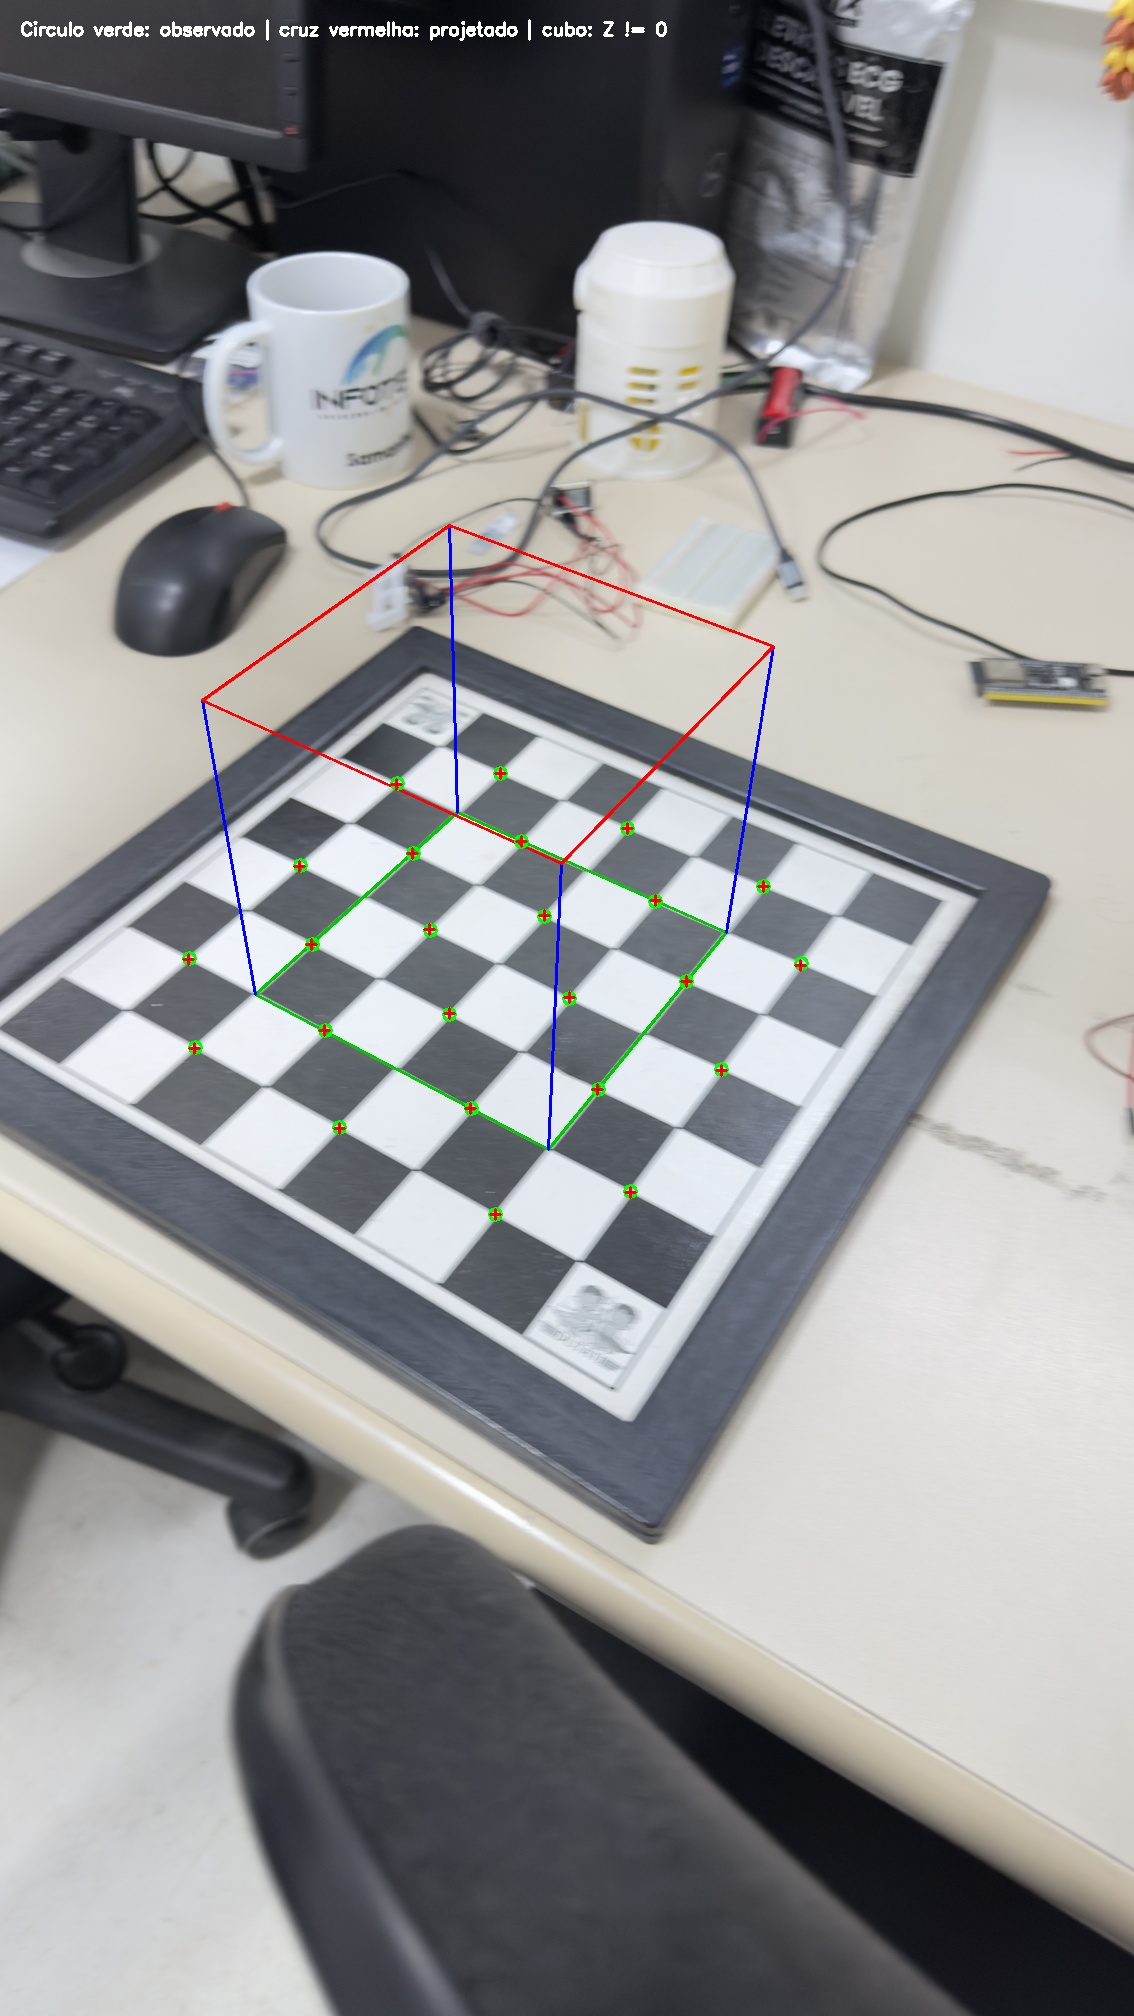
\includegraphics[height=7.2cm]{projecao_IMG_8174.jpg}
  \caption{Esquerda: IMG\_8157 original e sem distorção (linhas amarelas de
  referência). Direita: IMG\_8174 com cantos observados (círculo verde),
  projetados (cruz vermelha) e cubo projetado.}
  \label{fig:resultados}
\end{figure}

\section*{Discussão}

Os pontos projetados ficam, em média, a menos de 1~px dos cantos detectados em
fotos que não entraram na calibração. O maior erro é em IMG\_8165, que tem
reflexos fortes sobre o tabuleiro. A correção da distorção reduziu a curvatura
das linhas em todas as fotos de validação, mas pouco, porque o iPhone já
entrega a foto quase sem distorção.

Limitações: poucas vistas de calibração muito inclinadas (2 de 10 passam de
30°; 4 ficam abaixo de 10°), o tabuleiro nunca perto das bordas da imagem e o
lado do quadrado sem medida. Os erros estão em pixels e não medem a precisão 3D
em milímetros.

\vspace{-6pt}
\begin{thebibliography}{9}\small
\bibitem{zhang} ZHANG, Z. A flexible new technique for camera calibration.
  \emph{IEEE TPAMI}, v. 22, n. 11, p. 1330--1334, 2000.
\bibitem{opencv} OPENCV. Camera Calibration.
  \url{https://docs.opencv.org/4.x/dc/dbb/tutorial_py_calibration.html}.
\bibitem{todt} TODT, E. Camera Model and Calibration. Slides da disciplina,
  UFPR, 2026.
\end{thebibliography}

\end{document}
